% !TeX root = ../libro.tex
% !TeX encoding = utf8

\chapter{Resultados principales}

\section{Enunciados}
	\begin{teora}
		Toda variedad topológica 2-dimensional tiene una estructura diferenciable.
	\end{teora}

	\begin{teorb}
		Todo homeomorfismo entre variedades diferenciables 2-dimensionales es isotópico a un difeomorfismo.
	\end{teorb}
	
	Suponiendo ciertos los teoremas anteriores, es directa la obtención del siguiente resultado, ya que por A tenemos que toda variedad topológica 2-dimensional tiene una estructura diferenciable y por B sabemos que es única salvo difeomorfismos:
	
	\begin{corolario} (Teorema clásico de Munkres)
		Toda variedad topológica 2-dimensional tiene una única estructura diferenciable salvo difeomorfismos.
	\end{corolario}

\section{Demostración del Teorema A}

	\begin{teora}
		Toda variedad topológica tiene una estructura diferenciable.
	\end{teora}
	\begin{proof}[Demostración]
		Sea S una variedad topológica sin borde, podemos coger un sistema coordenado de cartas finito $\{(V_i, h_i)/ 1\leq i\leq N\}$. Vamos a construir por inducción una estuctura diferenciable en el conjunto $U_n = \cup_{i\leq n}h_i(\mathbb{R}^2)$, que por ser un sistema coordenado su límite debe de ser S, probando así el resultado. Cabe destacar que cada $U_i$ contiene a todos los anteriores. \\
		\\ La inducción empieza tomando una carta cualquiera del sistema, $U_1=V_1$ por ejemplo. Si se considera la variedad $U_1$ con el atlas $\{(h_1,U_1)\}$ entonces $h_1$ es diferenciable para ésta de forma trivial (se compone con la inversa y queda la identidad en $\mathbb{R}^2$).\\
		\\ Una vez arrancada la inducción, suponiendo cierto para el paso $n-1$ vamos a extender la diferenciabilidad de $U_{n-1}$ a $U_n$. Sea la carta $(V_n, h_n)$, tomamos entonces $W=h_n^{-1}(U_{n-1})=h_n^{-1}(U_{n-1}\cap h_n(V_n))$, que es un abierto de $\mathbb{R}^2$ por ser $h_n$ un homeomorfismo de $\mathbb{R}^2$ a $V_n$. \\
		\\ Tenemos $W\subset V_n$ abierto en $\mathbb{R}^2$, por el \textbf{Hecho 1} sabemos que existe una triangulación geométrica suya y que al ser abierto (no tiene borde) al ir acercándose al borde los triángulos tienden a ser puntos. Queremos aplicar el ``Teorema de alisamiento de asas'' en los vértices de los triángulos, seguidamente en los lados y finalmente en el interior de cada uno (aplicar los 3 apartados del teorema de forma consecutiva), pero para ello es necesario partir de un embebimiento de $\mathbb{R}^2$:
		\begin{enumerate}
			\item Para cada vértice $p$, elegimos una bola abierta lo suficientemente pequeña de forma que sus cierres no se corten (lo hacemos para todos los vértices de una vez), $B(p,\varepsilon _p)\subset W$ que es difeomorfo a $\mathbb{R}^2$ ($f_p:\mathbb{R}^2\rightarrow B$ difeomorfismo, con $f_p(0)=p$). Tomamos $g=h_n\circ f_p:\mathbb{R}^2\rightarrow h_n(W)$, que es un embebimiento por serlo $h_n|_B:B\rightarrow h_n(W)$ y $f_p$ (la composición de embebimientos es un embebimiento). \\
			\\ Aplicamos el apartado 1 del Teorema de alisamiento de asas y obtenemos una $\widehat{g}$ isotópica a la primera, que es diferenciable en $O_p$ (entorno abierto del origen, con $0=f_p^{-1}(p)$) y además queda fija fuera de otro entorno un poco mayor $O_p'\supset O_p$, con $\overline{f_p(O_p)}\subset B $. Si tomamos la función a trozos $\widehat{h}_n|_{B}=\widehat{g}\circ f_p^{-1}$ y $\widehat{h}_n|_{W-B}=h_n$, está bien definida porque en $B-f_p(O_p)$ al aplicar $f_p^{-1}$ nos lleva a $\mathbb{R}^2-O_p$, que es donde $\widehat{g}=g$, es decir: \\
			\begin{center}
				$\widehat{h}_n|_{B-f_p(O_p)}=\widehat{g}\circ(f_p^{-1}|_{B-f_p(O_p)})=g\circ(f_p^{-1}|_{B-f_p(O_p)})=h_n|_{B-f_p(O_p)}$\\
			\end{center}
			por lo que la función a trozos está bien definida, es diferenciable entorno a $p$ y no se altera fuera de $B$. \\
			\\ Éste paso se puede realizar de forma simultánea para todos los vértices, obteniendo así una $\widehat{h}_n$ que es diferenciable entorno a todos los vértices y se mantiene $h_n$ fuera de un entorno de cada vértice, algo mayor que el anterior (entornos con cierres disjuntos). Es por ello que para no cargar demasiado la notación se llamará a esa nueva función $h_n$.
			\item Tenemos un $h_n$ que es diferenciable entorno a los vértices de los triángulos y queremos usar el apartado 2 del Teorema de alisamiento de asas para extender la diferenciabilidad a un entorno tubular de los lados de los triángulos. Para ello, vemos que en cada lado, junto con los entornos de los vertices, podemos incluir un rectángulo abierto (conjunto abierto de $W$) que contenga a todo el segmento y cuyos segmentos laterales del rectángulo estén contenidos en ambas bolas. Este conjunto es difeomorfo a $\mathbb{R}^2$ y aplicando previamente dicho difeomorfismo cumplimos las hipótesis deseadas.\\
			\\ Al proseguir de forma semejante al apartado anterior, conseguimos una función $h_n$ que es diferenciable en un entorno del conjunto de todos los lados, quedando fija fuera de un entorno algo más grande.
			\item Buscamos finalmente una curva dentro del``esqueleto'' de entornos de los lados de los triángulos que junto con su componente interior sea difeomorfa a la bola cerrada unidad, para aplicar el 3$^{er}$ apartado del Teorema de alisamiento de asas y así obtener una $h_n$ diferenciable en todo $W$.\\
			\\ La curva buscada debe ser diferenciable, cerrada y simple, para así decir que es una curva de Jordan y aplicar el Teorema de la curva de Jordan. Como consecuencia, sabemos que su componente interior es difeomorfa a la bola unidad de $\mathbb{R}^2$. Podemos reducir el problema a buscar dicha curva para el entorno tubular de un triángulo equilátero, ya que es difeomorfo al de un triángulo cualquiera. Además, podemos seguir simplificándolo, aportando únicamente una curva no cerrada cuyos extremos se puedan pegar consecutivamente, siendo infinitamente derivable en los puntos donde se unen.\\
			\\ Haciendo uso de una función meseta $f$ que vale $0$ en $\mathbb{R}^-$ y $1$ a partir de $\epsilon > 0$, si tomamos $g(x)=tg(\frac{\pi}{3})xf(x)$ en el intervalo $[-1,\epsilon]$, tenemos que $g(-1)=0$ y $g(\epsilon)=tg(\frac{\pi}{3})\epsilon$  al igual que sus derivadas, por lo que si vamos alternando $g(x)$ y $g(-x)$ mediante rotaciones y traslaciones, tendremos una curva $\alpha$ diferenciable (suavización del triángulo equilátero). \\
			%\newpage
			\begin{figure}[h]
  				\centering
  				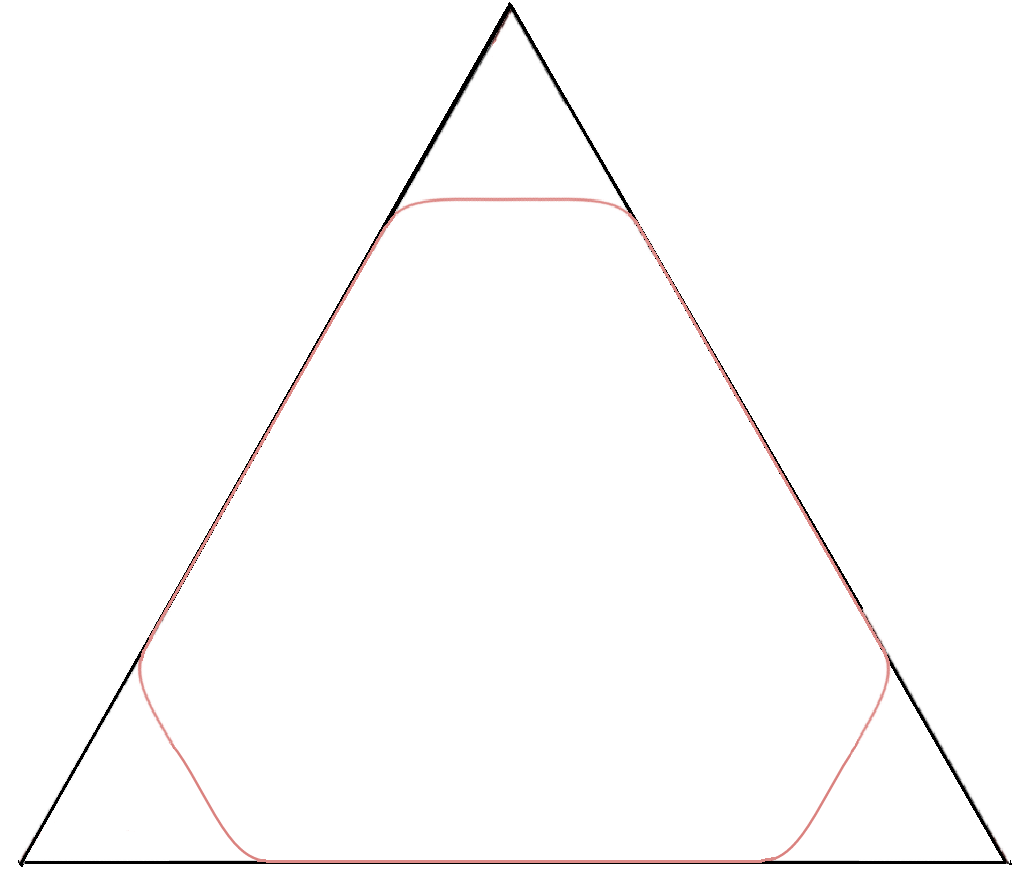
\includegraphics[width=0.5\textwidth]{triangulo_suavizado}
  				\caption{Curva de Jordan cercana al triángulo}
  				\label{fig:triangulo_suavizado}
			\end{figure}
			\\ Se puede observar que es válido $\forall \epsilon > 0$ y que al hacer tender $\epsilon$ a $0$, la curva será el propio triángulo equilátero. Es por ello que podemos tomar el $\epsilon$ lo suficientemente pequeño como para que la curva $\alpha$ quepa en el entorno tubular y siga siendo una curva de Jordan. \\
			\\ Ya tenemos un difeomorfismo entre la bola unidad y la componente interior de cada uno de los triángulos, que contienen un abierto conexo en el cual la función no es todavía diferenciable. Estamos en las condiciones del punto 3 del Teorema de alisamiento de asas, así que procediendo de igual forma que en los apartados anteriores obtenemos una $h_n$ totalmente diferenciable en $W$.
		\end{enumerate}
		
		Cabe destacar que en el borde de $W$ la aplicación se queda intacta, ya queen todo momento se está trabajando en el interior de $W$ (es abierto) y en todo paso de la "suavización" de $h_n$ siempre se deja inalterado el espacio complemento de un entorno mayor al aquel donde se obtiene la diferenciabilidad. Es por ello que se puede extender el $h_n$ obtenido a todo $\mathbb{R}^2$ junto con el original, porque está bien definido, quedando intacta en $\mathbb{R}^2-W$. 
	\end{proof}

\section{Demostración del Teorema B}
	\begin{teorb}
		Todo homeomorfismo entre variedades diferenciables 2-dimensionales es isotópico a un difeomorfismo.
	\end{teorb}
	\begin{proof}[Demostración]
		Sea $f: S \rightarrow S'$ homeomorfismo entre variedades diferenciales 2-dimensionales, se pueden dar 2 casos:
		\begin{enumerate}
			\item $\partial S = \phi$, por lo que podemos utilizar el \textbf{Hecho 2}, que nos aporta una triangulación diferenciable. Si utilizamos el mismo sistema coordenado que para la demostración del Teorema A, al aplicar $h_i^{-1}$ a dicha triangulación diferenciable, por definición tenemos una triangulación clásica en $\mathbb{R}^2$. Si componemos $f$ con $h_i$ ($g=f\circ h_i$), tenemos un embebimiento $g: \mathbb{R}^2 \rightarrow S'$.\\
			\\ Aplicando los apartados del Teorema de alisamiento de asas conseguimos un embebimiento diferenciable $\widehat{g}$ isotópico a $g$, y tomando $\widehat{f}=\widehat{g}\circ h_i^{-1}$ tenemos un homeomorfismo diferenciable isotópico a $g\circ h_i^{-1}=f$. De forma simétrica, aplicándolo a $\widehat{f}^{-1}$, obtenemos que $f$ es isotópico a un difeomorfismo. 
			\item $\partial S \neq \phi$, podemos considerar un collar diferenciable de $\partial S$ en $S$ e isotopar f a a un homeomorfismo diferenciable cerca del borde, dentro de ese conjunto, independientemente del difeomorfismo elegido para el collar diferenciable. Dicha isotopía se obtendrá utilizando el Teorema de alisamiento de asas, tal y como se ha hecho en el apartado anterior. La isotopía dejará fija a $f$ fuera del collar diferenciable. Lo hacemos de igual forma para la inversa, obteniendo una isotopía que deja fija a $f^{-1}$ fuera de un collar diferenciable del borde de $S'$, siendo diferenciable en otro collar diferenciable contenido en el anterior.\\
			\\ Ahora partimos de un homeomorfismo diferenciable en el borde de $S$, aplicando lo utilizado en el apartado anterior podemos obtener una isotopía a $\widehat{f}$, que es un difeomorfismo de $S$ a $S'$,ya que se puede tomar una triangulación en los interiores de las superficies (entendemos por interior a la superficie menos su borde). Aplicamos los mismos pasos para la inversa de $\widehat{f}$, obteniendo así que $f$ es isotópico a un difeomorfismo en todo $S$.
		\end{enumerate}
	\end{proof}
\endinput
%------------------------------------------------------------------------------------
% FIN DEL CAPÍTULO. 
%------------------------------------------------------------------------------------
